\documentclass{Head}
\begin{document}
\tableofcontents
\linenumbers
\section{Introduction}
Macromolecules are characterized by their long-chain structure, including molecular chain unit and conformation on the angstrom scale, lamella on the nanometer scale and spherulites on the micron scale.
Nowadays, synchrotron radiation small angle X-ray scattering (SAXS) and wide angle X-ray diffraction (WAXD), as a non-destructive, highly statistically averaged structure analysis method, have been extensively used in crystalline polymer research area.
For instance, information on grains in crystalline polymer, micro-domains in blended polymers and the shape, size and distribution of cavities and cracks can be obtained by guinier scattering.
Information on orientation, thickness and crystalline fraction of crystalline layer and the thickness of the amorphous layer can be obtained by long-period measurement.
\begin{figure}
    \centering
    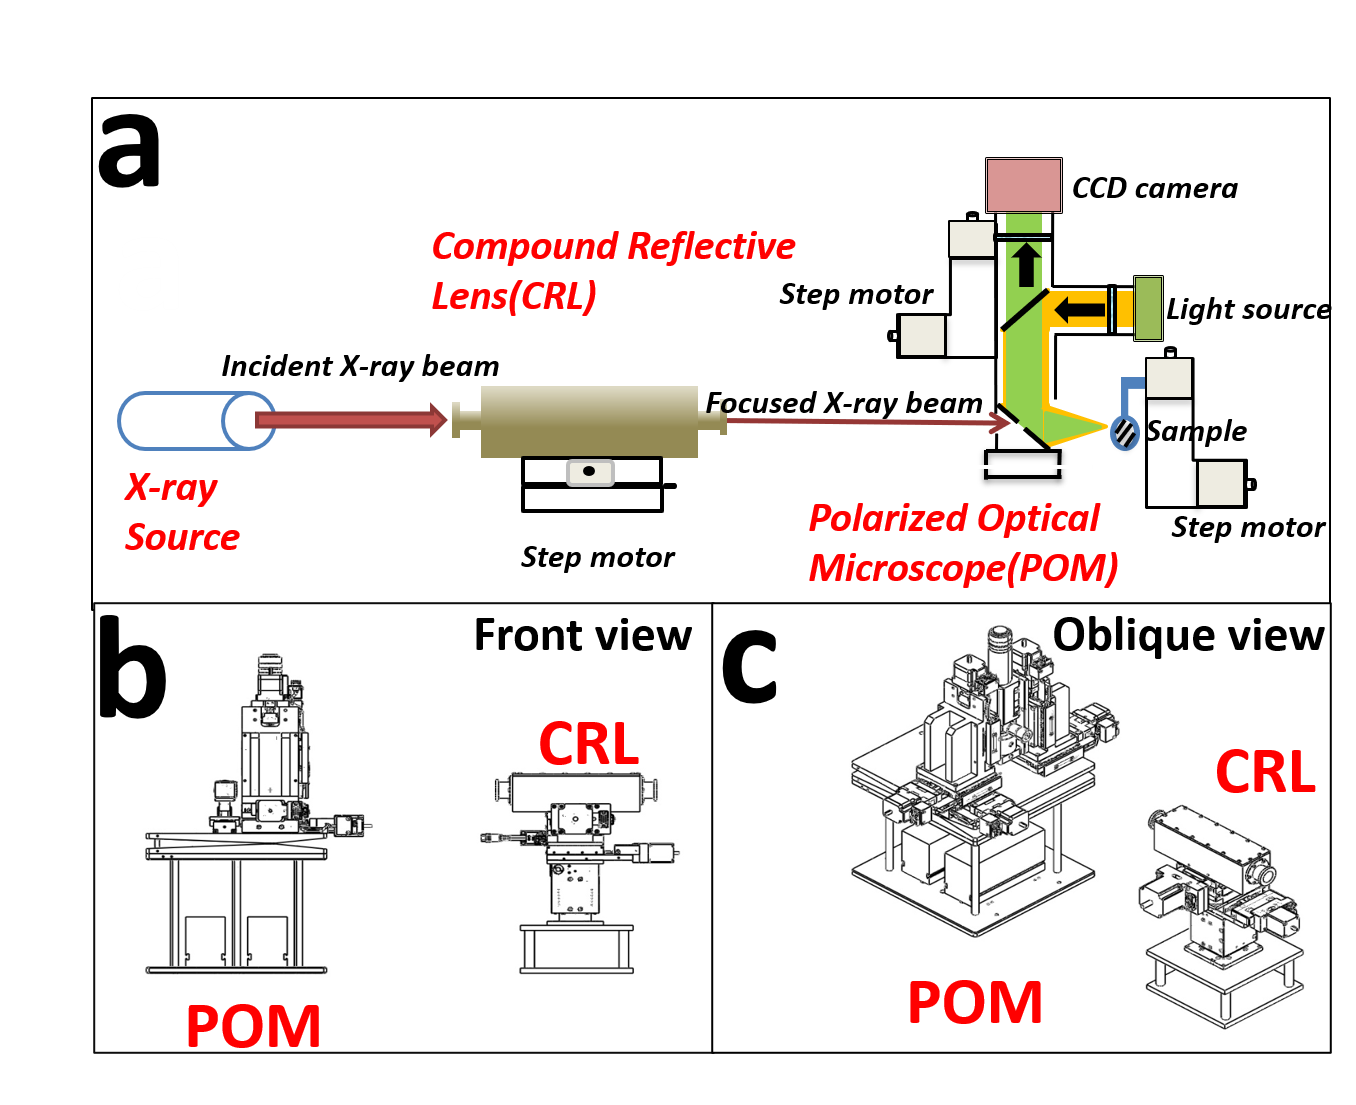
\includegraphics[scale=0.5]{Figures/Fig1WholeSystem.png}
    \caption{Whole system.}
    \label{WholeSystem}
\end{figure}


To further study the internal structure of polymers, two test conditions are essential.
Firstly, considering the size of specific structural unit, the size of the X-ray spot can not be too large.
For instance, in spherulites research, an X-ray spot with a size of 5$\mu$m$\times$5$\mu$m is required.
A small spot provides sufficient spatial resolution when the structure of macromolecules are characterized by the SAXS method.
Secondly, to match the characterization result with the real structure, it is a critical measure to confirm the real-time exact position of the X-ray incident beam on polymer crystal.


As described, the X-ray spot needs to be focused and located.


To improve the spatial resolution of the synchrotron radiation experiment, nearly all the world’s advanced synchrotron radiation facilities focus the X-ray spot in the micron or even sub-micron level.
Representative beam line stations include PETRA \uppercase\expandafter{\romannumeral3} P03, SSRF BL15U1.
However, limited by the distance between the sample and the detector, SAXS experiments can not be implemented on these stations.
Consequently, it is necessary to build an independent optical system with the functions of X-ray micro-focusing and precise spot positioning on the existing SAXS beam line.


The main component used for X-ray beam focusing includes a Kirkpatrick-Baez mirror, Fresnel zone plates, Capillary optical lens and Compound refractive lenses.
In synchrotron radiation area, Kirkpatrick-Baez mirror(K-B mirror) and Compound refractive lenses(CRL) are more widely used.
In practice, advantages of K-B mirror are aberration-free imaging on both horizontal and vertical planes, no dispersion, high energy, high reflectivity and low flux losses.
However, there are some non negligible disadvantages.
Micro-beam focusing by K-B mirror needs to be achieved by adjusting the interval mirrors and multi-axis spatial attitude, including: the angle of incident X-ray on the mirrors, the vertical angle of the two mirrors, spatial parallelism of two vertical cylinders.
The deployment of K-B mirror changes the original optical path.
Thus, the K-B mirror, as an off-axis device, increases the complexity of the installation of all the experimental equipment.
This is unfavorable for the entire micro-focusing experiment process.


Compound refractive lenses(CRL) are comprised of a series of single lenses arranged in a linear array to achieve X-ray focusing in the energy range of 5-40 keV.
As shown in \autoref{CRL}, the most widely used CRL are parabolic CRL.
The parabolic CRL has a parabolic surface that rotates around the axis of symmetry to form a parabola.
It can focus X-rays in two dimensions without causing aberrations in theory.
Compared to K-B mirror, CRL does not alter the original optical path propagation direction. CRL has excellent high temperature stability, simple and compact structure and low requirements for lens' surface roughness. Moreover, CRL is not difficult to adjust and relatively insensitive to vibration.
The most obvious disadvantage of CRL is its low transmission efficiency.
Owing to the small aperture of the diaphragm and the high absorbed rate of X-ray for CRL, the intensity of focused light will drop by one to two orders of magnitude than original light.
Despite this, the luminous flux can be maintained at $\mathrm{10^{10}\sim 10^{11} phs/s}$ after CRL micro-focusing.
It can be proved in \autoref{CRL parameter determination}.
This flux is enough for the structure research of crystalline polymers.
\begin{figure}
    \centering
    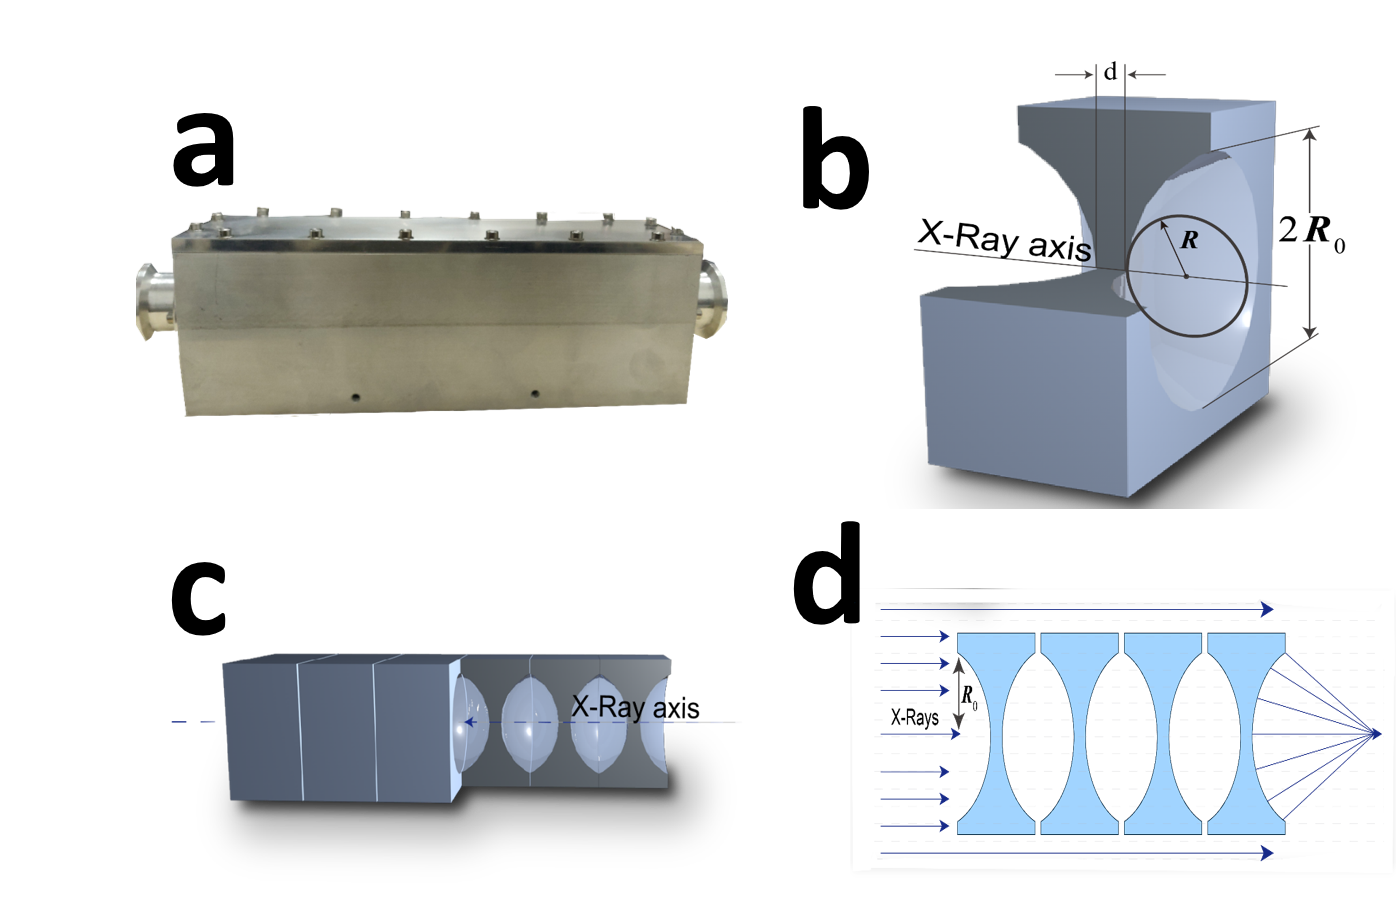
\includegraphics[scale=0.4]{Figures/Fig2CRL.png}
    \caption{Structure of Compound reflective lenses}
    \label{CRL}
\end{figure}


Polarized optical microscopy(POM) is commonly used in polymer crystal morphology research.
POM is a simple method to distinguish the change of growth direction of crystals in the film plane and to check whether there exists twisting of crystals\cite{RN37}.
\autoref{POM} is a schematic diagram of the disassembly of a POM.
When the polarized light generated by the polarizer and the analyzer enters the anisotropic polymer crystal, birefringence occurs, and the crystal contrast is provided by the coherence of the polarized light.
Different crystal forms of polymers, such as spherulites, string crystals, stretched chain crystals, transverse crystals, etc., all have anisotropic optical properties, so their crystal morphology, size, number, etc. can be observed clearly with a POM.
\begin{figure}
    \centering
    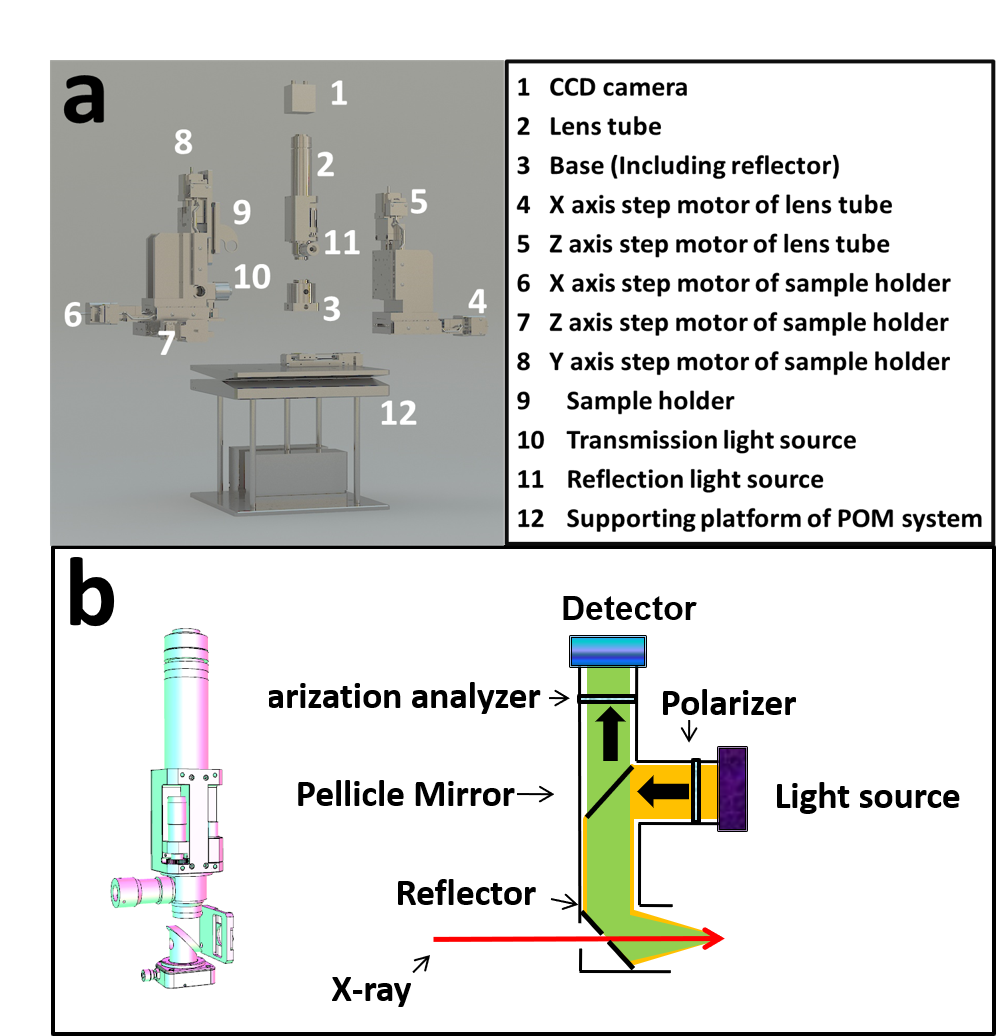
\includegraphics[scale=0.4]{Figures/Fig3POM.png}
    \caption{POM overall disassembly and lens cone disassembly.}
    \label{POM}
\end{figure}


In this passage, a combined system of micro-focusing SAXS and POM is proposed.
A series of parameters of the device is adjusted, and the device is used to characterize the crystalline morphology and microstructure of related polymers.
\section{Experiment}
\subsection{Construction of stable light path}
\subsubsection{CRL parameter determination}
\label{CRL parameter determination}
In order to obtain the designed X-ray microbeam, CRL's parameters are necessary to be determined first.
The parameter mainly include material, geometric size and number of pieces.
Commonly used CRL is aluminum and beryllium.
Basing on the theory of atomic physics, materials with low atomic number have less absorption of X-rays. In this system, a beryllium CRL is chosen because the X-ray energy has to be preserved as much as possible.



There are three common single lenses.
The main geometric parameters of them are listed in \autoref{CRL parameters}.
First, CRL with a radius of 50 $\mathrm{\mu m}$ is selected to calculate the relevant parameters.
\begin{table}
    \centering
    \caption{Parameters of several common single lens}
    \begin{tabular}{ccc}
        \toprule
        Radius $R$/$\mathrm{\mu m}$ & Aperture 2$R_0$/$\mathrm{\mu m}$ & Area $\pi R_0^2$/$\mathrm{mm^{-2}}$ \\
        \midrule
        200                         & 881                              & 0.609                               \\
        100                         & 623                              & 0.305                               \\
        50                          & 440                              & 0.152                               \\
        \bottomrule
    \end{tabular}
    \label{CRL parameters}
\end{table}


Transmittance refers to the ratio of the light intensity after passing through the lens and the light intensity without passing through the lens.
It can be calculated by \autoref{transmission equation}\cite{Lengeler:ht2006}:
\begin{equation}
    T_p=\frac{\int_0^{2\pi}\mathrm{d}\theta\int_0^{R_0}e^{-\mu ND(r)}r\mathrm{d}r}{\int_0^{2\pi}\mathrm{d}\theta\int_0^{R_0}r\mathrm{d}r}=\frac{1-e^{-a}}{a}e^{-\mu Nd}
    \label{transmission equation}
\end{equation}
In \autoref{transmission equation}, $a=\mu N R_0^2/R$, $R$ and $R_o$ are given in \autoref{CRL parameters}, $N$ is the number of lens, $d$ is the minimum thickness of a single mirror.
For parabolic lenses, d can be calculated by \autoref{width}:
\begin{equation}
    D(r)=d+2\times \frac{r^2}{2R}
    \label{width}
\end{equation}
The maximum thickness $D(r)$ of the selected CRL is 2 mm.
Substituting $D(r)$ and $r=R_0$ into the \autoref{width}, d equals 1.032 mm.



Considering the actual situation of shed size and pipeline layout, the designed image distance is about 400 mm and so is the focal length.
The focal length under the approximate condition of thin lens can be calculated by \autoref{focal} :
\begin{equation}
    f=R/2N\delta
    \label{focal}
\end{equation}
N is the amount of lenses, $\delta$ is real part of refractive index to 1 offset.
$\delta$ can be calculated by \autoref{delta} \cite{als2011elements}:
\begin{equation}
    \delta=\frac{2\pi\rho r_o}{k^2}
    \label{delta}
\end{equation}
$\rho$ is electron number density, $r_o$ is the electronic classical radius and $k$ is wave vector.
For beryllium in 12KeV, $\delta$ is $2.36393\times 10^{-6}$.
When N is set to 30, the focal length is 352.5 mm.
This value meets the requirements described above.
Substituting $N=30$ and $d=1.032$ into the \autoref{transmission equation}, $T_p$ equals 0.327.


The flux of photons after passing through the lenses can be calculated by the following equation:
\begin{equation}
    I=i\times T_p \times R
    \label{intensity}
\end{equation}
$i$ is the flux of incident X-ray.
In BL19U2, under a current intensity of 220 mA, $i=2.5\times 10^{12}$ photons/s, $R$ is defined as the photon acceptance rate and equals 0.0598 in BL19U2.
Substituting these values into the \autoref{intensity}, $I$ equals $4.89\times 10^{10}$ photons/s. This value is enough to study the structure of crystalline polymers.


For lens with a radius of 100$\mu$m and 200$\mu$m, after the same calculation, N is 60 and 120.
Although a lens with a larger radius of curvature can be used to obtain a slightly larger flux, the number of lenses required is greatly increased.
Comprehensive consideration, using 30 lenses with a radius of 50 $\mu$m is the best choice.
\subsubsection{Reduce beam jitter}
Due to the thermal load caused by the high-power beam to the monochromator crystal and the vibration of the monochromator crystal caused by the liquid nitrogen cooling system of the monochromator, the current spot of the BL19U2 is differed by about 10\%, which will affect the strength stability of X-ray micro beam.


A processing software is compiled which integrates light intensity position data collection, data processing (calculation of beam center), data smoothing and filtering, PID control algorithm and control interface.
Advanced FPGA technology is applicable to design and implement a fuzzy adaptive PID controller.
Beam position which is collected by the PID control loop in real time is compared with the set value.
Then the comparison error is sent to the PID controller to calculate the control value through the PID control algorithm.
Subsequently, the comparison error is input to the actuator of the monochromator piezo to adjust the piezo angle of the second crystal in real time. This operation realizes the constant feedback system of the beam center position and the constant light intensity feedback system.
Finally, it is realized that the closed-loop control of the beam position and suppress low the beam drift of the frequency band to realize the stabilization of the BL19U2.
Thus, the impact of beam jitter on the intensity of the focused beam is lowered.
\subsection{Construction of the combined system}

\autoref{WholeSystem} is the schematic diagram of the structure of synchrotron radiation X-ray micro-focusing polarized microscopy system.
The combined system has one micro-focusing component and an in situ polarized light microscope system.
After the incident X-ray is focused by the CRL, it will pass through the light hole on the lower side of the POM and the sample, then the scattered signal will be received by the detector.
The on-site construction diagram of the system is shown in \autoref{sitemap}.
\begin{figure}
    \centering
    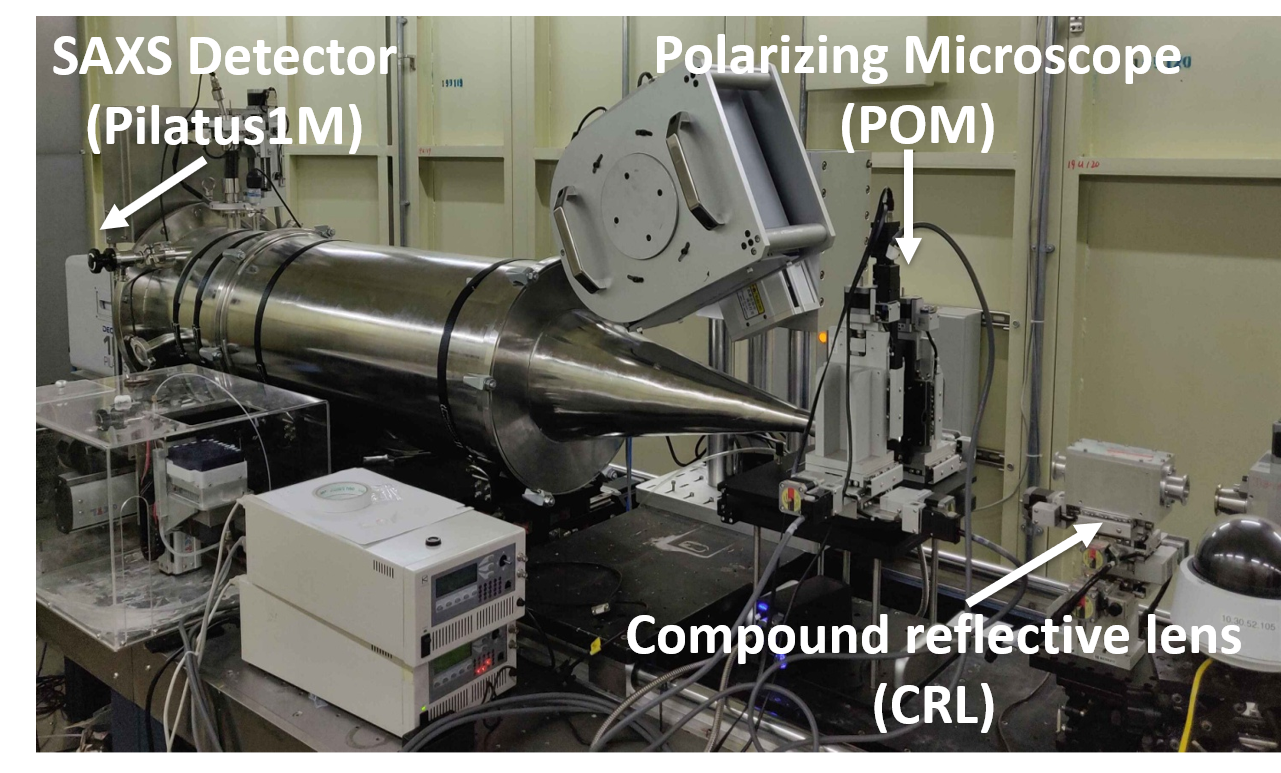
\includegraphics[scale=0.5]{Figures/Fig4SiteMap.png}
    \caption{Site map of the combined system.}
    \label{sitemap}
\end{figure}

As shown in \autoref{WholeSystem}, the CRL is mounted on a motorized platform. Including three-dimensional translational electric platform (x, y, z three directions), one-dimensional swing stage (P angle) and one-dimensional rotating platform (R angle). The posture of CRL can be adjusted in five spatial dimensions.


The structure of POM used in the system is shown in \autoref{POM}.
As shown in \autoref{POM}b, the optical system of POM mainly consists of the following parts: a polarizer and analyzer that use ordinary white light sources to generate polarized light; a half mirror located in the middle of the lens barrel; A flat mirror located at the bottom of the lens barrel. The detector at the top is utilized to collect images. In this system, the detector selects a Charge-coupled device(CCD) camera.


As shown in \autoref{POM}a, the in situ POM system is also installed on a motorized support platform.
A stepping motor (4$\sim$5) installed on the side of the lens body realizes the translational adjustment of the lens barrel in two dimensions.
Similarly, the stepping motor (6$\sim$8) on the side of the sample holder realizes its translational adjustment in three dimensions.
The supporting platform (12) can be further divided into three layers: the uppermost layer is a one-dimensional swing stage and a rotating table, the middle layer is a two-dimensional (horizontal) translational electric platform, and the lowest layer is a three-dimensional translational electric platform.
Through the adjustment devices in all the above dimensions, the five spatial dimensions of the entire optical system can be adjusted.
\subsection{Determination of spot parameters}
Once the combined system is installed in beam line, the beam can be adjusted.
The main purpose of beam adjustment is threefold: first, to ensure the connectivity of the integrated optical path, to ensure that X-rays can pass through the system correctly.
A series of elements on the fixed light path of the beam line is used to adjust the primary light spot, and then the light path is adjusted using the POM and CRL spatial dimensions.
The current value of the ionization chamber can determine whether there is sufficient X-ray flux to irradiate the sample.
The second purpose is to verify whether the CRL is accepted to focus the primary spot to a sufficiently small spot size.
Only when the size is basically in line with the theoretical value to achieve a sufficiently small spatial resolution, can the microstructure of the research system be characterized; the third is to adjust the position of the light spot to the center of the field of view, while adjusting the angle of the plane mirror to make the polarized light that reaches the sample after being reflected twice by the half mirror and the plane mirror is focused on the X-ray at this point in the sample.
The detection point of the sample is placed in the center of the field of view, and the detection position will not shift even if the magnification of the polarizing microscope is changed.
To achieve the latter two purposes, we need to observe the spot in real time under POM.
For this reason, we install a cesium iodide crystal on the sample stage. Cesium iodide crystal has the characteristic of emitting fluorescence under X-rays, so it is also called scintillation crystal. In this system, the X-ray spot position is calibrated by the fluorescence spectrum generated by cesium iodide under POM.
\begin{figure}
    \centering
    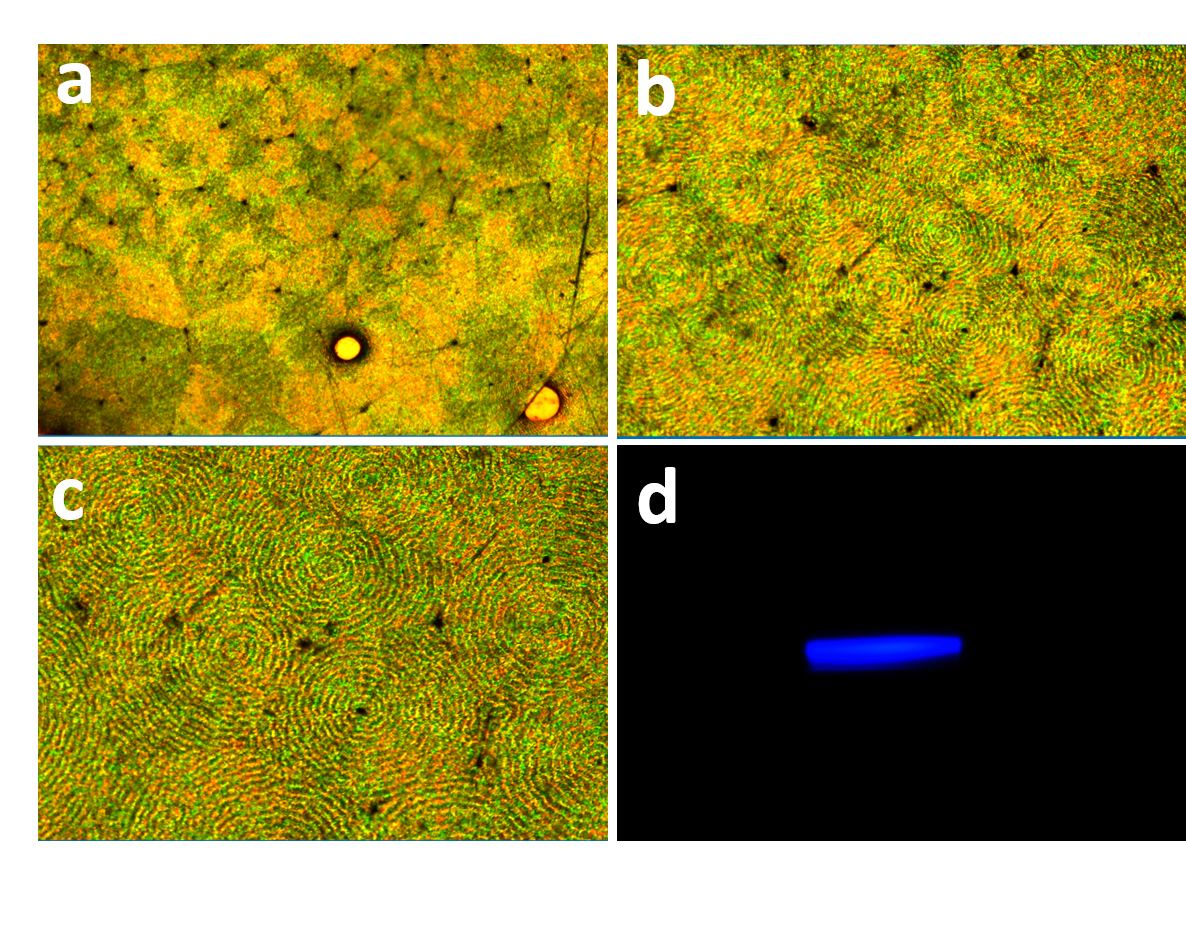
\includegraphics[scale=0.5]{Figures/Fig5CommissionPOMOnSite.png}
    \caption{Result of commissioning POM on site}
    \label{pictures}
\end{figure}


Step motors used in this system are all produced by Kohzu Corporation.
Positioning accuracy can reach 1um, which is enough for precise spatial position adjustment.
Adjust the CRL posture so that the incident X-ray can pass through the lenses correctly and be focused.
Then adjust the y-direction motor of the POM sample stage, so that the scintillation crystal is correctly focused and imaged in the field of view of the polarizing microscope.
Finally, set the x and z direction motors to move the center of the field of view to the fluorescent spot.
In the PC imaging software, a cross ruler will be displayed to provide assistance in positioning.



The theoretical size of the focus spot is about 5$\mu$m$\times$ 5$\mu$m.
In check to see whether the error between the actual size and the theoretical calculation is within the allowable range, two methods are used.
As shown in \autoref{fitting}a and \autoref{fitting}b, the first is to visually observe through imaging software and use a ruler to make rough measurements.
This method is fairly intuitive and fast, but the accuracy is insufficient.
The second method is Gaussian fitting by using current data of ionization chamber.
Basing on related theories, the flux of X-rays determines the intensity of the current in the ionization chamber.
FWHM of the $\frac{\mathrm{d}I}{\mathrm{d}x}\sim x$ curve(first derivative of the ionization chamber current to displacement) represents the spot size.
Representative fitting results of this system are shown in \autoref{fitting}c and \autoref{fitting}d.
The FWHM of the fitted peak is calculated to be 5.43$\mu$m$\times$6.52$\mu$m.
This value basically achieves the expected effect.
\begin{figure}
    \centering
    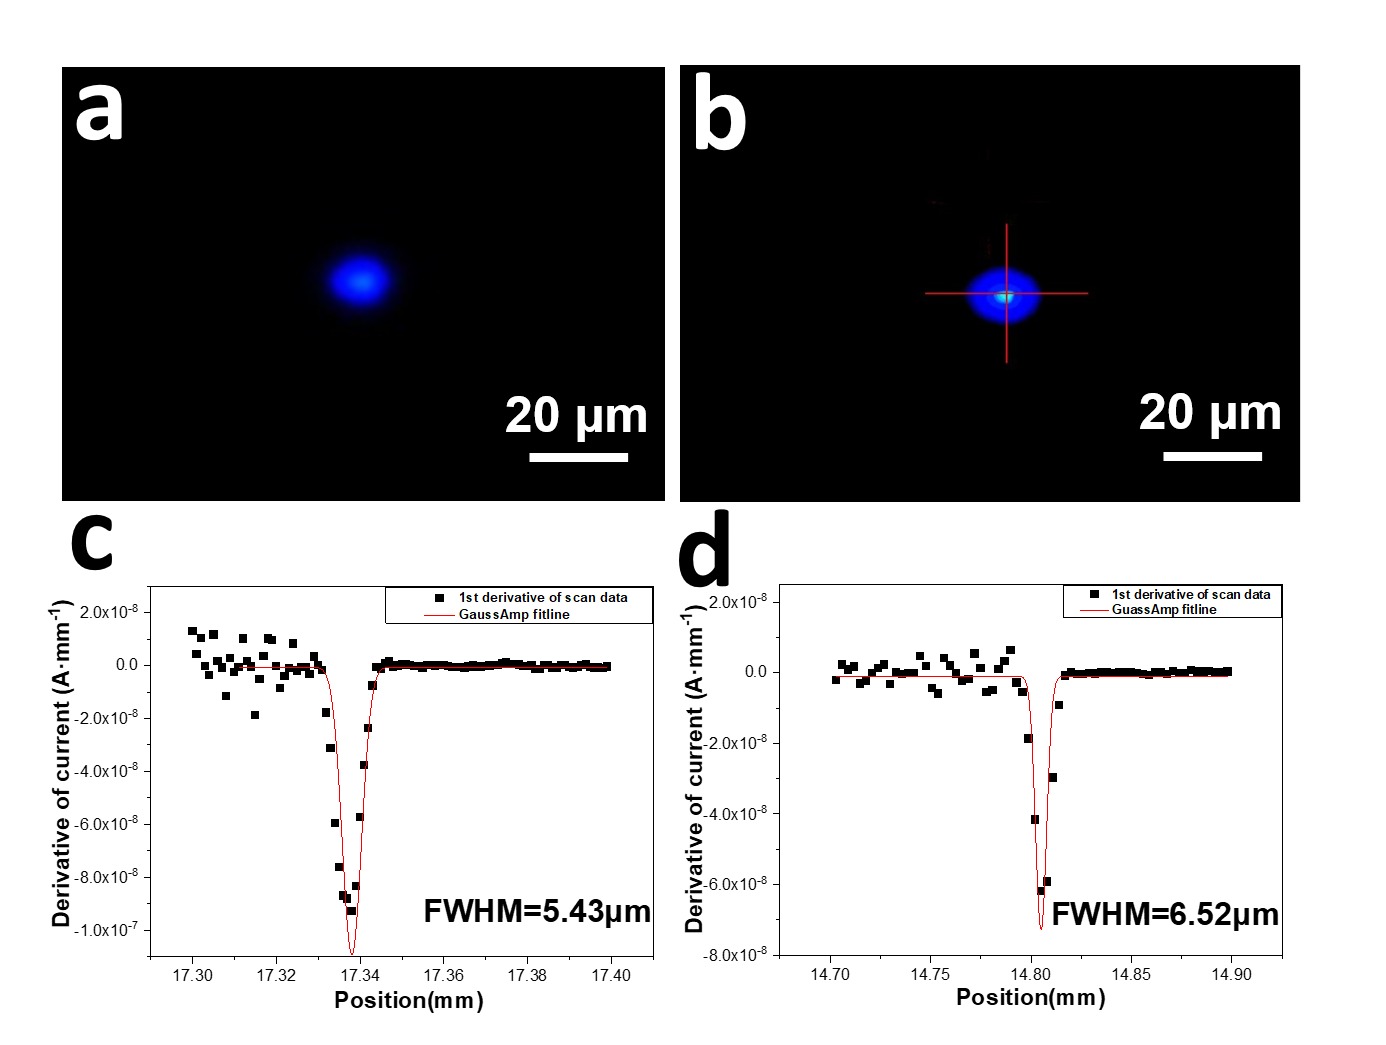
\includegraphics[scale=0.5]{Figures/Fig6CRLmicrofocus.png}
    \caption{Result of CRL micro-focus (facula and flux)}
    \label{fitting}
\end{figure}
\subsection{Collection of micro-focus X-ray scattering data}
After adjusting the size and position of the light spot, it can be utilized to characterize the micro-domain structure of related polymer crystals.
First, determine the position that needs to be characterized under the POM, and then use the motor installed on the platform to remove the visible light source. Passing in synchrotron X-rays to collect scattered signals.
At the SSRF-BL19U2 line station, X-rays with an energy of 12keV are often utilized, and the distance between the sample and the detector is 2700mm.
The scattering signal is collected by Pilatus1M detector (981$\times$1043pixel, with a pixel size of 172$\mu$m$\times$172$\mu$m).


\section{Application}
In order to verify the feasibility of the entire combined system, the spherulites with annulus and fibers with a sheath-core structure are used as research examples.
Micro-focused X-ray spot is used for micro-area resolution, and the scattering information of small structures that cannot be obtained by ordinary small-angle scattering experiments can be obtained.
\subsection{Microstructure of ringed sperulites}
Spherulites are the most common morphological structure of polymer materials, and they play a vital role in the physical, chemical and mechanical properties of polymer materials. Its multi-level structure is complicated, and many basic scientific issues related to its structure have yet to be further explored.
At present, in the study of the microstructure of zonal spherulites, there are several scientific problems that need to be explained urgently. The first problem is the correlation between the growth axis of the polymer ring-belt spherulites and the torsion chirality of the lamellae.
One theory is that the growth axis affects the chirality of the lamella torsion by changing the pressure distribution on the lamella plane.
Micro-focus X-ray can be used to determine the growth axis of each region and the tilt torsion behavior of the mapping crystal plane along the growth axis, revealing the correlation between the crystal growth axis and the lamella torsion chirality. It can provide a scientific basis for clarifying the transfer behavior of chirality between the multi-level structure of polymer spherulites.
The second problem is the cross nucleation of polymer spherulites during the crystallization.
Through micro-focus X-ray, the crystalline transformation information at the front of spherulite growth are monitored in situ, including crystal plane, orientation, whether there is a transition (gradient) zone to reveal the cross nucleation mechanism in polymer crystals, and clarify multiple crystal types the correlation and the similarities and differences between polymer cross nucleation and traditional cross nucleation of small molecule.
\begin{figure}
    \centering
    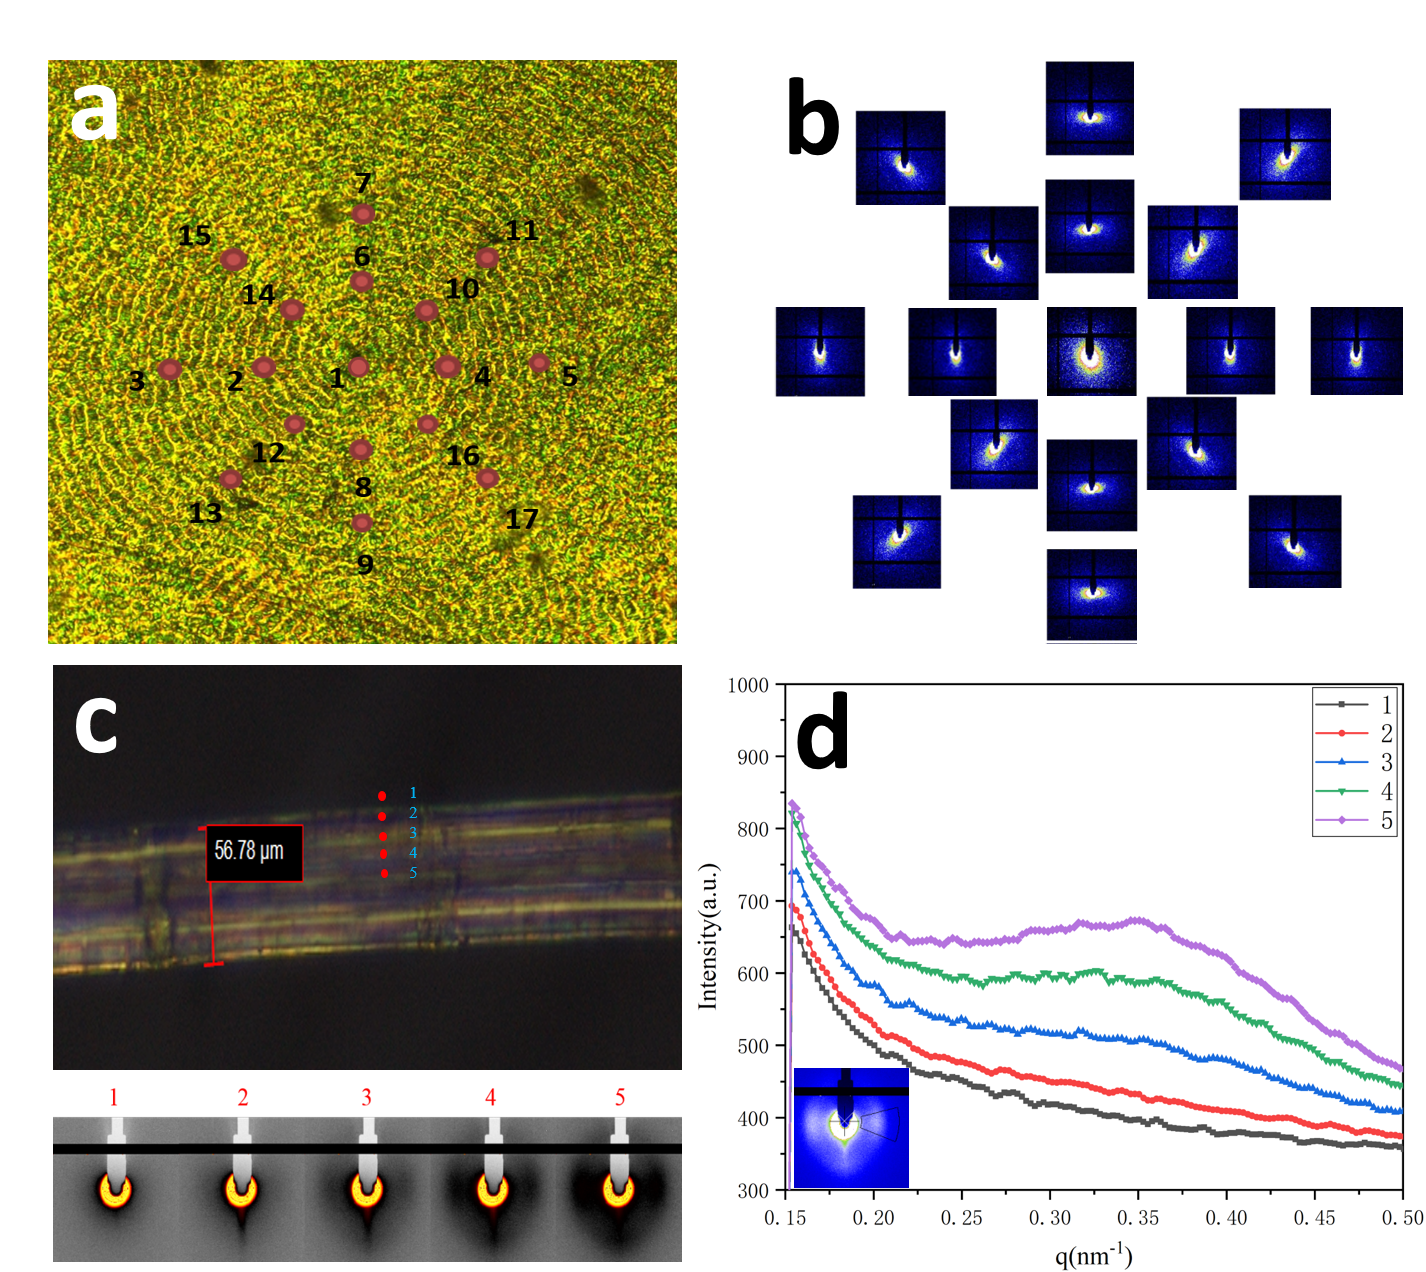
\includegraphics[scale=0.4]{Figures/Fig7AppliedResearch.png}
    \caption{The application sample of the system}
    \label{apply}
\end{figure}


Ringed-spherulites were chosen to verify the usability of the micro-focusing polarizing microscope system.
Micro beam X-ray scans were especially informative. As shown in \autoref{apply}a, the initial growth site (1) of the ringed-spherulites was first calibrated, and the micro-focus SAXS characterization was performed on this point.
Subsequently, 8 sites were uniformly selected and characterized on a certain circumference of the ring-belt spherulites.
In order to eliminate contingency, a total of 16 sites (2-17) in two different circles were selected, and SAXS characterization was also performed.
The two-dimensional image of the SAXS result is shown in \autoref{apply}b, and it can be seen from \autoref{apply}b that the distribution of the scattering intensity at different sites is different. The scattering intensity at the center of the spherulites is equal in all directions.
However, in all directions around the ringed-spherulites, there is a certain orientation, which also reflects the periodic changes in the arrangement of the lamellae on the ringed-spherulites.
Through the precise characterization of the ringed-spherulites by micro-focused X-rays, experimental results with certain differences have been obtained. The above examples can support the usability of the system.
\subsection{The skin and core structure of the fiber}
For fiber materials, the skin layer and the core layer of the fiber will have certain structural differences due to the temperature and shear flow field factors in the preparation process.
Some fibers have small diameters, and conventional SAXS methods cannot accurately characterize the structure of the skin or core layer.
The interval of taking points is about 5$\mu$m
Micro-focused X-rays can accurately distinguish the skin layer from the core layer and even the transition layer, and use the scattering data to study the structural differences.


As shown in \autoref{apply}c, the micro-beam X-rays irradiate the detection points of the skin and core of the fiber. The corresponding scattering data is shown in \autoref{apply}d.
\section{Conclusion}
In this paper, based on the development trend of multi-scale structure characterization methods of polymer materials, for the first time, a set of CRL-POM combined device was built on a synchrotron radiation line station to realize the scattering characterization based on optical micro-area resolution. The research methods and technical routes used in this experiment have been tested many times. The feasibility of the experimental system has also been verified by a variety of material research systems. The system can provide theoretical guidance for the molecular structure and high-performance design of related materials in the industry. At the same time, it also provides a new characterization platform for the SSRF Small angle X-ray scattering station, and a new combination structure characterization method for internal and external teams conducting polymer crystal structure research.
\bibliography{reference.bib}
\end{document}